\section{Modelagem do SMO}

A validação do observador seguiu três etapas: simulação com os parâmetros
medidos do motor (\autoref{tab:parametros_simulacao}), ajuste automático dos
ganhos e aplicação aos registros de bancada (\autoref{sec:ensaios_bancada}).
Na simulação (\autoref{fig:diagrama_blocos_smo}), a planta do inversor de seis
passos (\autoref{fig:diagrama_planta}) gera as grandezas de referência,
chamadas aqui de ``dados reais''. O SMO (\autoref{fig:diagrama_smo}) estima a
força contraeletromotriz bruta, e um PLL extrai dela o ângulo e a velocidade,
a partir dos quais a força contraeletromotriz é reconstruída analiticamente.
Essa reconstrução substitui a forma clássica, de arco-tangente com filtro
passa-baixas, cujo atraso de fase fazia o estimador perder o sincronismo nas
desacelerações.

\begin{table}[htbp]
    \centering
    \caption{Parametros para simulação}
    \label{tab:parametros_simulacao}
    \begin{tabular}{lcc}
        \toprule
        \textbf{Parâmetro} & \textbf{Símbolo} & \textbf{Valor} \\
        \midrule
        Resistência de fase     & $R_s$    & \num{17,3} \si{m\Omega} \\
        Indutância de fase      & $L_s$    & \num{7} \si{\micro\henry} \\
        Polos                   & $P$      & \num{14} \\
        Pares de polos          & $p$      & \num{7} \\
        Constante de velocidade & $K_v$    & \num{310} \si{RPM/V} \\
        Momento de inércia      & $J$      & \num{0,0001} \si{kg.m^2} \\
        Coef. de carga --- APC 15x6E\footnotemark
                                & $k_{Q}$  & \num{1,00e-6} \si{N.m/(rad/s)^2} \\
        Coef. de carga --- APC 17x10E
                                & $k_{Q}$  & \num{2,61e-6} \si{N.m/(rad/s)^2} \\
        Tensão do barramento    & $V_{bus}$& \num{30} \si{V} \\
        Período de amostragem   & $T_s$    & \num{10e-6} \si{s} \\
        Tempo de simulação      & $t_{end}$& \num{10} \si{s} \\
        \bottomrule
    \end{tabular}

    \footnotetext{Carga da hélice $T_{carga}=k_Q\,\omega_m^2$, com
    $k_Q = C_Q\,\rho\,D^5/4\pi^2$ e $C_Q$ médio do fabricante entre
    \num{1000} e \num{3000} RPM \cite{apc_performance_data}.}

    Fonte: Autor (2026)
\end{table}


\begin{figure}[H]
    \centering
    \caption{Diagrama de blocos do sistema de estimação híbrido com reconstrução analítica de BEMF.}
    \label{fig:diagrama_blocos_smo}
    \vspace{0.3cm}
    \begin{tikzpicture}[
        auto, node distance = 2.5cm,
        block/.style={rectangle, draw, thick, text width=3.5cm, text centered, minimum height=1.5cm, font=\small},
        line/.style={draw, thick, -{Stealth[length=2.5mm, width=1.5mm]}},
        coord/.style={coordinate}
    ]
        \node [block] (motor) {Planta Dinâmica \\ Máquina BLDC};
        \node [block, right=2cm of motor] (clarke) {Transformada \\ de Clarke};
        \node [block, right=2cm of clarke] (smo) {Observador \\ Modos Deslizantes \\ (SMO)};
        \node [block, below=1.5cm of smo] (pll) {Extrator de Fase \\ (PLL)};
        \node [block, left=2cm of pll] (recon) {Reconstrutor \\ Analítico BEMF};
        \node [block, left=2cm of recon] (torque) {Cálculo de \\ Torque ($\hat{T}_e$)};
        \draw [line] (motor) -- node [above] {$i_{a,b,c}$} (clarke);
        \draw [line] (clarke) -- node [above] {$i_{\alpha}, i_{\beta}$} (smo);
        \draw [line] (smo) -- node [right] {$\hat{e}_{\alpha, raw}, \hat{e}_{\beta, raw}$} (pll);
        \draw [line] (pll) -- node [above] {$\hat{\theta}, \hat{\omega}$} (recon);
        \draw [line] (recon) -- node [above] {$\hat{e}_{\alpha, cln}, \hat{e}_{\beta, cln}$} (torque);
        \coordinate (mid_clarke_smo) at ($(clarke.east)!0.5!(smo.west)$);
        \draw [line, dashed] (mid_clarke_smo) -- ++(0,-1.5) -| node [near end, left] {$i_{\alpha}, i_{\beta}$} (torque.north);
    \end{tikzpicture}
    \vspace{0.3cm} \\
    \small Fonte: Autor (2026).
\end{figure}


\begin{figure}[htbp]
    \centering
    \caption{Planta do inversor somente para simulação.}
    \label{fig:diagrama_planta}
    \vspace{0.3cm}
    \begin{tikzpicture}[
        auto, node distance = 2.5cm,
        block/.style={rectangle, draw, thick, fill=white, text width=4.5cm, text centered, minimum height=1.5cm, font=\small},
        sum/.style={circle, draw, thick, fill=white, minimum size=6mm, text centered, font=\large},
        line/.style={draw, thick, -{Stealth[length=2.5mm, width=1.5mm]}}
    ]
        \node [coordinate] (input) {};
        \node [sum, right=1.5cm of input] (sum1) {$\Sigma$};
        \node [block, right=1cm of sum1] (pi) {Controlador PI (Vel.) \\ $V_{cmd} = K_{pw} e + K_{iw} \int e\, dt$};
        \node [block, right=1cm of pi] (inv) {Inversor (6-Passos) \\ Aplica $V_{act}$ ou $0$ a partir de $f_{PWM}$ e $\theta_e$};
        \node [block, below=1cm of inv] (motor) {Modelo BLDC (Elétrico)};
        \node [block, left=1cm of motor] (mec) {Dinâmica Mecânica};
        \draw [line] (input) -- node {$\omega_{ref}$} (sum1);
        \draw [line] (sum1) -- node {$e_\omega$} (pi);
        \draw [line] (pi) -- node {$V_{cmd}$} (inv);
        \draw [line] (inv) -- node {$v_{abc}$} (motor);
        \draw [line] (motor) -- node [above] {$T_e$} (mec);
        \draw [line] (mec) -| node [near end, right] {$\omega_m$} (sum1);
        \coordinate (out_i) at ($(motor.east) + (1cm, 0)$);
        \draw [line] (motor.east) -- node [above] {$i_{abc}$} (out_i);
        \draw [line, dashed] (mec.south) -- ++(0,-0.5) -| node [near start, below] {$\theta_e, \omega_m \rightarrow e_{abc}$} (motor.south);
    \end{tikzpicture}
    \vspace{0.3cm} \\
    \small Fonte: Autor (2026).
\end{figure}

A \autoref{fig:inversor_sim} mostra a resposta do controlador PI de velocidade da planta.

\begin{figure}[H]
    \centering
    \caption{Controlador PI para o inversor da planta (hélice 17x10E).}
    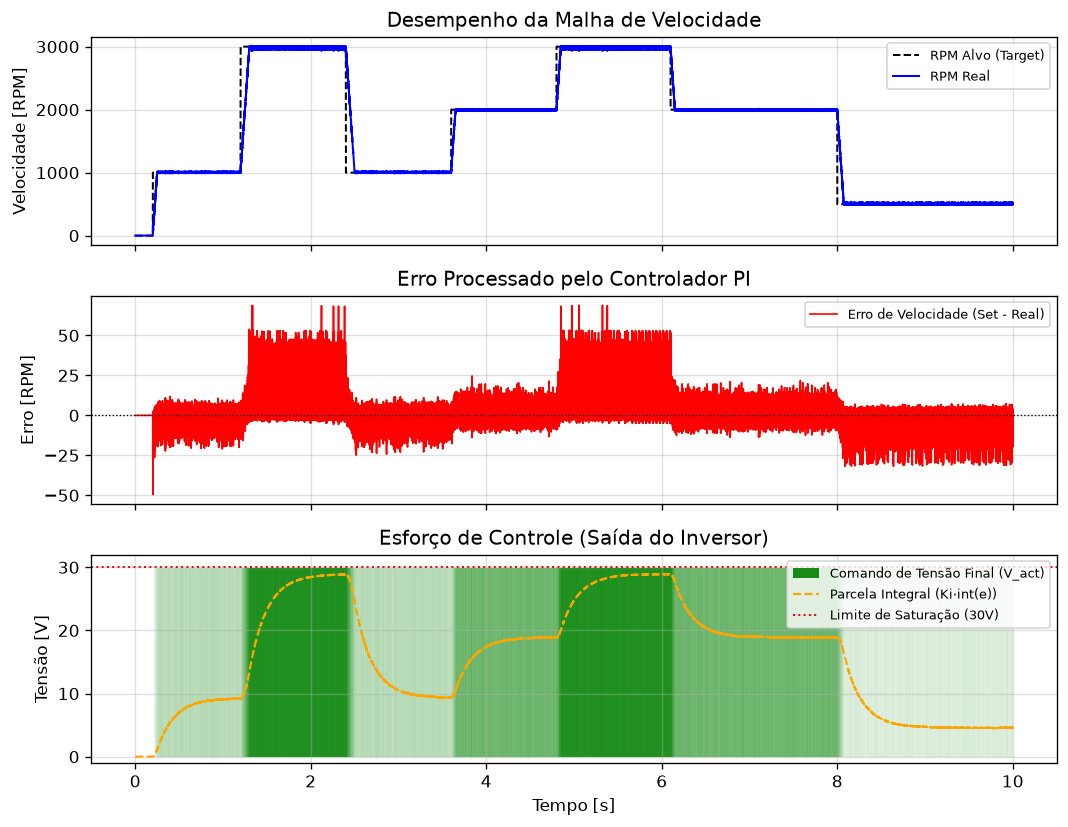
\includegraphics[width=0.9\linewidth]{Textuais/Imgs/Desenvolvimento/PI_controle_Inversor.png}
    \label{fig:inversor_sim}

    Fonte: Autor (2026)
\end{figure}

\begin{figure}[htbp]
    \centering
    \caption{Malha de estimação de corrente e Back-EMF.}
    \label{fig:diagrama_smo}
    \vspace{0.3cm}
    \begin{tikzpicture}[
        auto, node distance = 2.5cm,
        block/.style={rectangle, draw, thick, fill=white, text width=4.5cm, text centered, minimum height=1.5cm, font=\small},
        sum/.style={circle, draw, thick, fill=white, minimum size=6mm, text centered, font=\large},
        line/.style={draw, thick, -{Stealth[length=2.5mm, width=1.5mm]}}
    ]
        \node [coordinate] (in_i) {};
        \node [sum, right=1.5cm of in_i] (sum_i) {$\Sigma$};
        \node [block, right=1cm of sum_i] (sat) {Função de Chaveamento \\ $s_{\alpha\beta} = \text{Sat}\!\left(\frac{e_i}{8{,}0}\right)$};
        \node [block, right=1cm of sat] (gain_smo) {Ganhos Deslizantes \\ $K_{s1} \cdot T_s, \quad K_{s2} \cdot T_s$};
        \node [block, below=1cm of gain_smo] (est_i) {Integração da Corrente \\ $\hat{i}_k = \Phi_i \hat{i}_{k-1} + \Gamma_v u + \Gamma_{s1} s$};
        \node [block, left=1.5cm of est_i] (est_e) {Estimativa BEMF  \\ $\hat{e}_{raw} = \Phi_e \hat{e}_{k-1} + K_{s2} s$};
        \draw [line] (in_i) -- node {$i_{\alpha\beta}$} (sum_i);
        \draw [line] (sum_i) -- node {$e_{i}$} (sat);
        \draw [line] (sat) -- node {$s_{\alpha\beta}$} (gain_smo);
        \draw [line] ([xshift=1cm]gain_smo.south) -- node [right] {$+ \Gamma_{s1} s$} ([xshift=1cm]est_i.north);
        \draw [line] ([xshift=-1cm]gain_smo.south) -- ++(0, -0.6cm) coordinate (drop) -- node [above] {$+ K_{s2} s$} (drop -| est_e.north) -- (est_e.north);
        \draw [line] (est_i.south) -- ++(0,-1.5) -| node [near end, right] {$\hat{i}_{\alpha\beta}$} (sum_i.south);
        \draw [line] (est_e.east) -- node [above] {$\hat{e}_{raw}$} (est_i.west);
        \coordinate (out_e) at ($(est_e.south) + (0,-1cm)$);
        \draw [line] (est_e.south) -- node [right] {$\hat{e}_{\alpha\beta, raw}$ para o PLL} (out_e);
    \end{tikzpicture}
    \vspace{0.3cm} \\
    \small Fonte: Autor (2026).
\end{figure}


% =====================================================================
% SUBSEÇÃO — CONDICIONAMENTO ANALÓGICO
% =====================================================================
\subsection{Condicionamento Analógico e seu Impacto na Reconstrução}
\label{sec:condicionamento}

A robustez do observador depende diretamente da fidelidade dos sinais de
tensão e corrente entregues ao algoritmo, uma vez que o SMO extrai a posição
angular justamente da coerência entre a tensão aplicada e a corrente
resultante.

Um fator físico limita essa reconstrução, e decorre da própria natureza da
força contraeletromotriz. Como sua
amplitude é proporcional à velocidade ($\hat{e} = K_e\,\hat{\omega}_e$), em
baixas rotações o sinal de interesse torna-se pequeno frente ao ruído de
chaveamento do observador, degradando a relação sinal-ruído da reconstrução.
Esse comportamento explica por que o erro angular é sistematicamente maior no
patamar de menor velocidade.

% =====================================================================
% PLL
% =====================================================================
Para mitigar os erros observados na extração de fase, integrou-se um
\textit{Phase-Locked Loop} (PLL) ao algoritmo
(\autoref{fig:diagrama_pll_recon}). O PLL atua como um filtro dinâmico que
ignora o ruído harmônico da BEMF bruta e sincroniza a posição estimada
($\hat{\theta}$) e a velocidade ($\hat{\omega}_e$). O erro de fase é obtido
pela projeção cruzada da BEMF bruta estimada sobre a referência angular atual,
formulação que se reduz à expressão clássica em cosseno e seno no caso de BEMF
senoidal e permanece válida para formas trapezoidais.

\begin{figure}[H]
    \centering
    \caption{PLL e reconstrução analítica da Back-EMF.}
    \label{fig:diagrama_pll_recon}
    \vspace{0.3cm}
    \begin{tikzpicture}[
        auto, node distance = 2.5cm,
        block/.style={rectangle, draw, thick, fill=white, text width=4.5cm, text centered, minimum height=1.5cm, font=\small},
        sum/.style={circle, draw, thick, fill=white, minimum size=6mm, text centered, font=\large},
        line/.style={draw, thick, -{Stealth[length=2.5mm, width=1.5mm]}}
    ]
        \node [coordinate] (in_e) {};
        \node [block, right=1.5cm of in_e] (pd) {Detector de Erro de Fase \\ $\epsilon = \frac{g_\alpha \hat{e}_\beta - g_\beta \hat{e}_\alpha}{|\hat{E}|}$};
        \node [block, right=1cm of pd] (pi_pll) {Filtro de Loop (PI) \\ $\hat{\omega}_e = K_{p,pll} \epsilon + K_{i,pll} \int \epsilon$};
        \node [block, below=1cm of pi_pll] (integ) {Integrador de Fase \\ $\hat{\theta} = \int \hat{\omega}_e\, dt$};
        \node [block, left=1cm of integ] (recon) {Reconstrução Analítica \\ $\hat{e}_{\alpha ,\beta} = K_e \hat{\omega}_e f_{\alpha,\beta}(\hat{\theta})$};
        \node [block, below=1cm of recon] (torque) {Equação de Torque \\ $\hat{T}_e = 1{,}5\, K_e\, p\, (\hat{e}_\alpha i_\alpha + \hat{e}_\beta i_\beta)$};
        \draw [line] (in_e) -- node [above] {$\hat{e}_{\alpha\beta, raw}$} (pd);
        \draw [line] (pd) -- node {$\epsilon$} (pi_pll);
        \draw [line] (pi_pll) -- node [right] {$\hat{\omega}_e$} (integ);
        \coordinate (loop_up) at ($(integ.east) + (1cm, 0)$);
        \coordinate (loop_top_right) at (loop_up |- {$(pd.north) + (0, 1.2cm)$});
        \coordinate (loop_top_left) at ($(pd.north) + (0, 1.2cm)$);
        \draw [line] (integ.east) -- (loop_up) -- (loop_top_right) -- node [above] {$\hat{\theta}$} (loop_top_left) -- (pd.north);
        \draw [line] (integ) -- node [above] {$\hat{\theta}$} (recon);
        \draw [line] (pi_pll.south) ++(-1cm,0) -- node [left] {$\hat{\omega}_e$} ($(recon.north) + (2cm,0)$);
        \draw [line] (recon) -- node [right] {$\hat{e}_{\alpha\beta, cln}$} (torque);
        \coordinate (in_i) at ($(torque.west) + (-1.5cm, 0)$);
        \draw [line, dashed] (in_i) -- node [above] {$i_{\alpha\beta}$ medida} (torque.west);
    \end{tikzpicture}
    \vspace{0.3cm} \\
    \small Fonte: Autor (2026).
\end{figure}

Quando a estimativa do PLL converge para a posição real do rotor, a componente
ortogonal do produto vetorial é forçada a zero, garantindo que $\hat{\omega}_e$
e $\hat{\theta}$ reflitam a dinâmica do eixo com forte imunidade ao ruído de
alta frequência. O desempenho do
sincronismo é apresentado na \autoref{fig:PLL_fig_desenvolvimento}.

\begin{figure}[H]
    \centering
    \caption{Performance do PLL (hélice 17x10E).}
    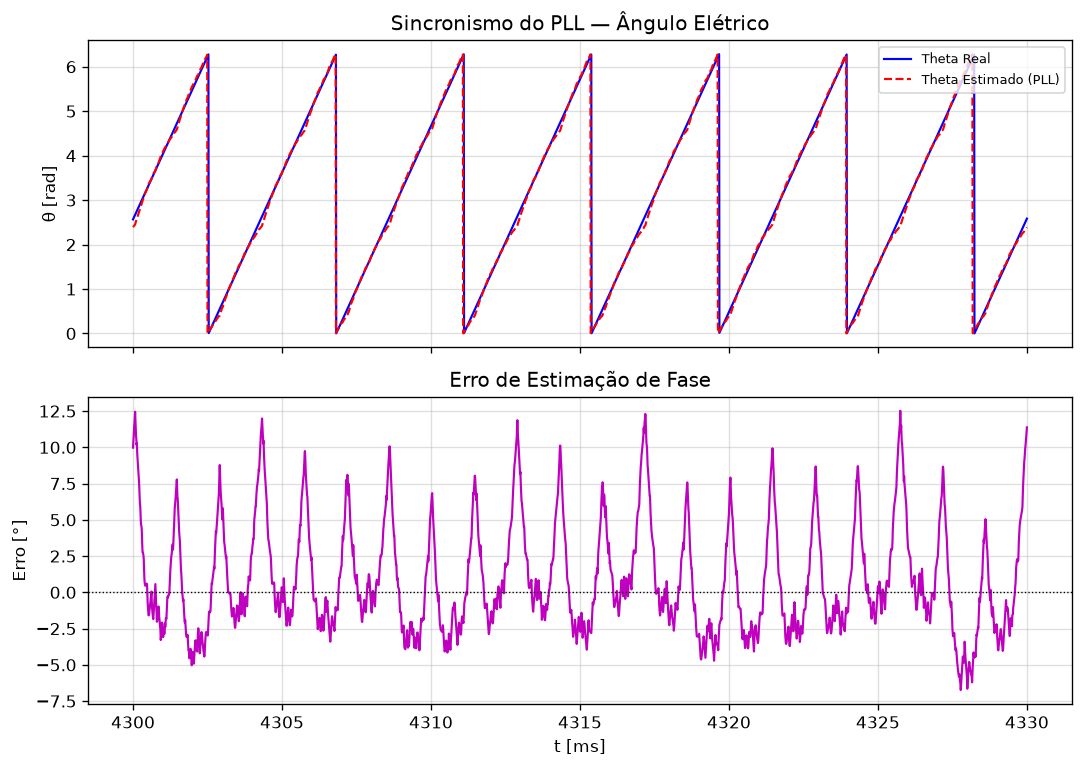
\includegraphics[width=0.7\linewidth]{Textuais/Imgs/Desenvolvimento/PLL_angulos.png}
    \label{fig:PLL_fig_desenvolvimento}

    Fonte: Autor (2026)
\end{figure}

% =====================================================================
% AUTOTUNING (subseção)
% =====================================================================
\subsection{Ajuste Automático dos Ganhos do Observador}
\label{sec:autotuning}

Aplicado o procedimento de \textit{autotuning} formulado na
\autoref{sec:param_smo}, a \autoref{fig:otim_convergencia} traz o custo de
cada avaliação e o melhor custo acumulado ao longo da busca, para a carga da
hélice 17x10E. O custo converge nas primeiras dezenas de avaliações e permanece
estável até o fim das cerca de \num{1000} avaliações. Os picos de três a quatro ordens de grandeza acima do patamar
correspondem a combinações de ganhos em que o observador diverge, visitadas
pela evolução diferencial durante a exploração do espaço de busca.


\begin{figure}[H]
    \centering
    \caption{Convergência da otimização dos ganhos do observador (hélice 17x10E).}
    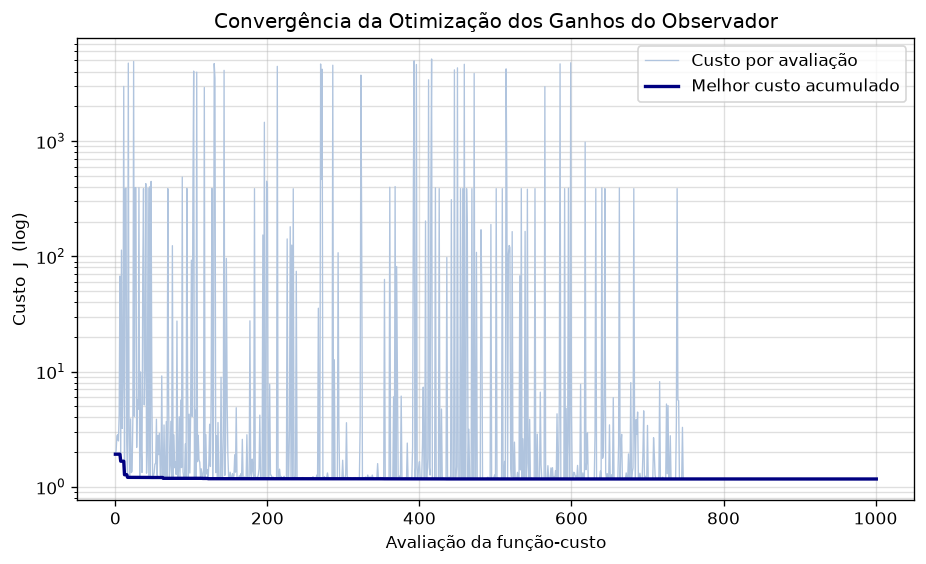
\includegraphics[width=0.85\linewidth]{Textuais/Imgs/Desenvolvimento/Otim_convergencia.png}
    \label{fig:otim_convergencia}

    Fonte: Autor (2026)
\end{figure}

Os ganhos obtidos para as duas hélices estão na
\autoref{tab:ganhos_helices}. $\Gamma_{s2}$ é o mesmo nas duas, no limite da
faixa de busca, e $\Gamma_{s1}$ muda pouco. Quem acompanha a carga é
$\Gamma_t$, ligado ao polo do estimador da \textit{Back-EMF}: com a 17x10E,
de torque maior, ele é cerca de 25 vezes o da 15x6E.

\begin{table}[H]
    \centering
    \caption{Ganhos do observador obtidos pelo ajuste automático, por hélice}
    \label{tab:ganhos_helices}
    \begin{tabular}{lcccc}
        \toprule
        \textbf{Hélice} & $\Gamma_{s1}$ & $\Gamma_{s2}$ & $\Gamma_t$ & \textbf{Custo final / inicial} \\
        \midrule
        APC 15x6E  & \num{20,73} & \num{-10,00} & \num{0,0037} & \num{1,013} / \num{1,300} \\
        APC 17x10E & \num{26,55} & \num{-10,00} & \num{0,095}  & \num{0,992} / \num{1,280} \\
        \bottomrule
    \end{tabular}

    \vspace{2pt}
    {\small Fonte: Autor (2026)}
\end{table}

Ao passo de simulação $T_s=\SI{10}{\micro\second}$, os ganhos da 17x10E
correspondem a $K_{s1}=\num{2,66e6}$, $K_{s2}=\num{-1,00e6}$ e
$K_t=\num{9,50e3}$. A otimização é conduzida sobre
$\Gamma = K\,T_s$ para que o resultado não fique preso ao passo de
integração: o \textit{firmware} recupera seus próprios ganhos dividindo os
mesmos $\Gamma$ pelo período de amostragem em que roda.

A \autoref{fig:otim_sensibilidade} apresenta a varredura unidimensional de
cada ganho em torno do ótimo, mantendo os demais fixos. Para $\Gamma_{s1}$, o
ponto encontrado fica no fundo de um vale. Para $\Gamma_{s2}$, fica no trecho
plano, perto da subida abrupta, de duas ordens de grandeza, que aparece com
ganhos maiores em módulo, onde a estimação deixa de acompanhar a planta.
$\Gamma_t$ quase não altera o custo, menos de \SI{1}{\percent} na faixa
varrida. $\Gamma_{s2}$ ficou no limite da faixa de busca, $|\Gamma_{s2}| \le 10$,
mas a varredura mostra que o custo é plano desse lado e só sobe com ganhos
maiores em módulo, então ampliar a faixa traria pouco ganho.

\begin{figure}[H]
    \centering
    \caption{Sensibilidade da função-custo aos ganhos do observador (hélice 17x10E).}
    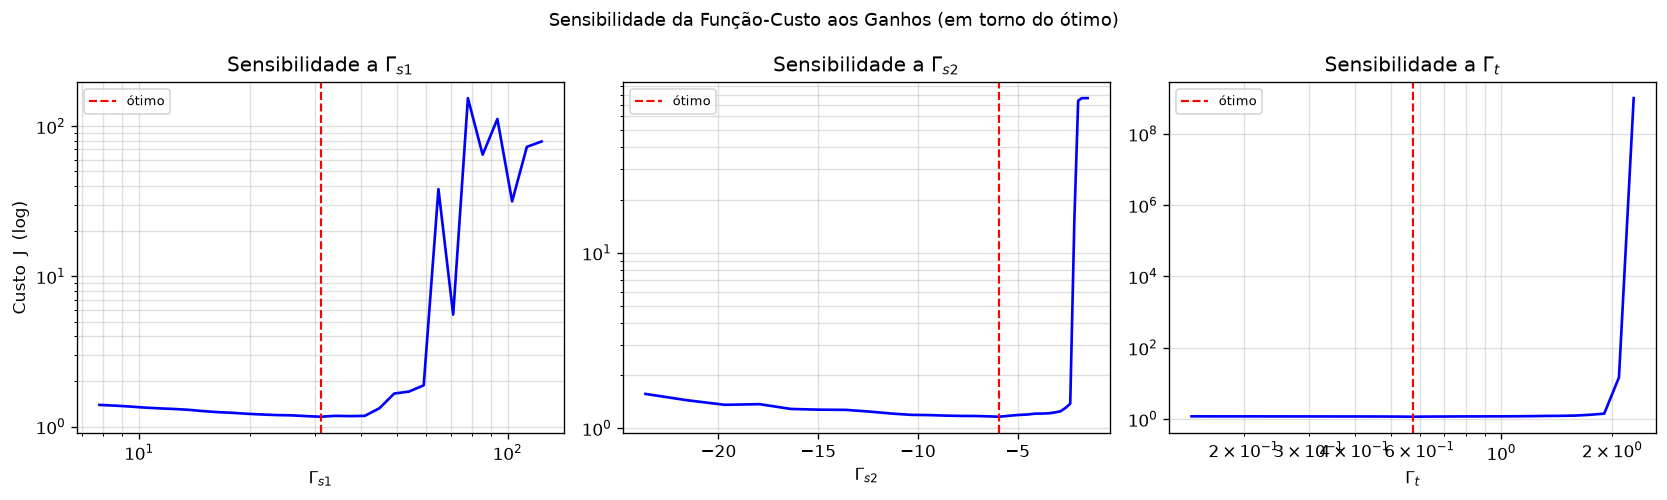
\includegraphics[width=\linewidth]{Textuais/Imgs/Desenvolvimento/Otim_sensibilidade.png}
    \label{fig:otim_sensibilidade}

    Fonte: Autor (2026)
\end{figure}

Em conjunto, a busca automática partiu de um ponto inicial arbitrário e chegou
a um conjunto de ganhos utilizável sem intervenção manual, com custo cerca de
\SI{22}{\percent} menor que o do ponto de partida nas duas hélices. Como o procedimento depende
apenas da resistência, da indutância e do perfil de velocidade adotado, pode
ser repetido para outro conjunto motopropulsor caracterizado na bancada.
% =====================================================================
% RESULTADOS MECÂNICOS E CONCLUSÃO
% =====================================================================

Com esses ganhos, a \autoref{fig:desempenho_mecanico} compara a rotação e o
torque estimados com os da planta ao longo do perfil de velocidade simulado,
para as duas hélices: patamares de \SIrange{1000}{5000}{RPM}, de
\SI{500}{RPM} em \SI{500}{RPM}, e uma desaceleração para \SI{3000}{RPM} no
fim. A rotação estimada acompanha os patamares, com atraso perceptível nas
transições, e na segunda metade de cada patamar fica a menos de
\SI{0,05}{\percent} da real. O torque instantâneo oscila cerca de
$\pm\SI{1}{\newton\meter}$, herdado do acionamento em seis passos; sua média,
obtida com o mesmo filtro passa-baixas de \SI{2}{\hertz} aplicado às saídas
do \textit{firmware}, sobe em degraus junto com a rotação, que é o torque da
hélice. Na 15x6E ela vai de \SI{0,030}{\newton\meter} a
\SI{0,306}{\newton\meter} e a estimada fica a menos de \SI{1,1}{\percent} da
real. Na 17x10E vai de \SI{0,047}{\newton\meter} a \SI{0,745}{\newton\meter}
e a estimada fica acima da real, de \SI{12}{\percent} no primeiro patamar a
\SI{4}{\percent} no último, diferença que diminui com a rotação, o que sugere
um erro que pesa mais quando o torque é pequeno. A \autoref{fig:eixos_estaticos} mostra,
em janela ampliada, as correntes e a força contraeletromotriz nos eixos
$\alpha$ e $\beta$: as grandezas estimadas seguem as reais, com o
\textit{chattering} característico do modo deslizante em torno delas.

\begin{figure}[H]
    \centering
    \caption{Rotação e torque reais e estimados ao longo dos patamares, por hélice}
    \label{fig:desempenho_mecanico}
    \begin{subfigure}[t]{\textwidth}
        \centering
        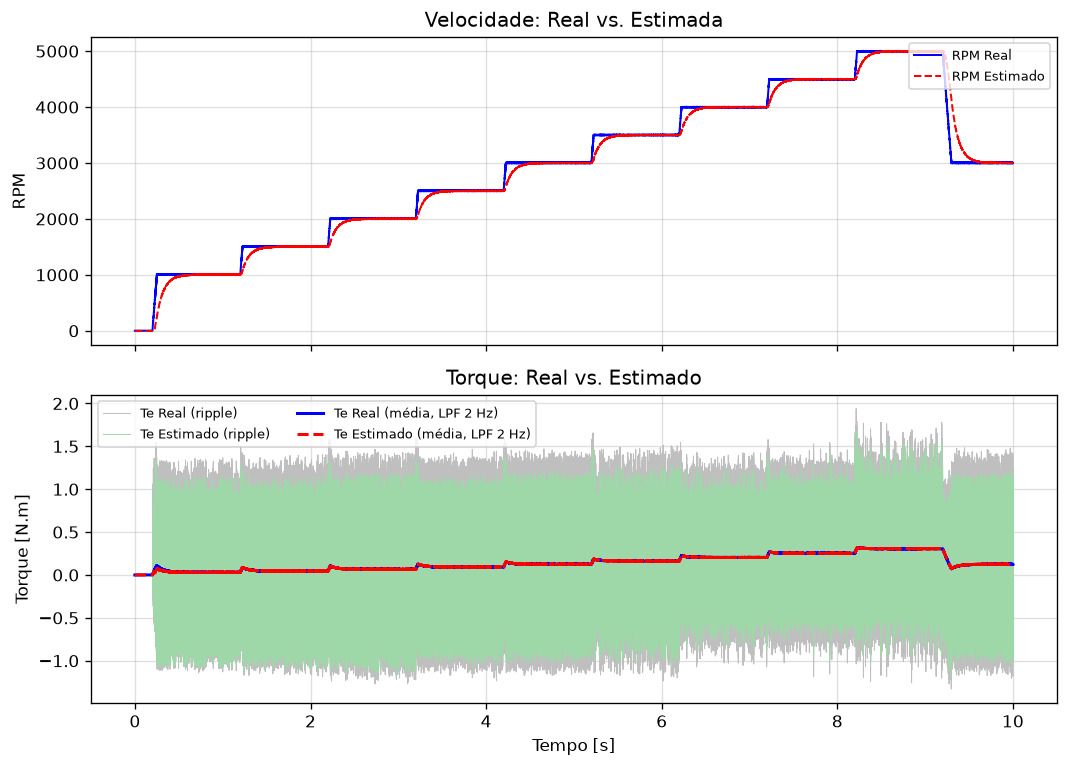
\includegraphics[width=0.8\linewidth]{Textuais/Imgs/Desenvolvimento/Torque_rpm_15x6E.png}
        \caption{APC 15x6E}
    \end{subfigure}

    \vspace{0.3cm}
    \begin{subfigure}[t]{\textwidth}
        \centering
        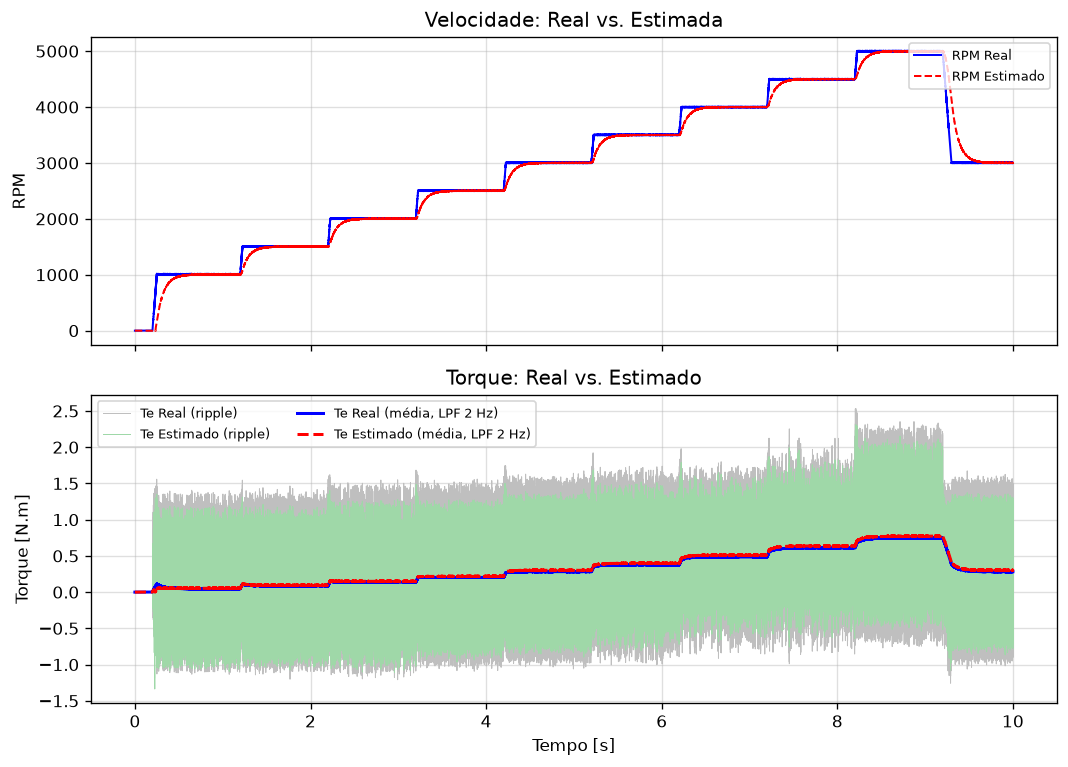
\includegraphics[width=0.8\linewidth]{Textuais/Imgs/Desenvolvimento/Torque_rpm_17x10E.png}
        \caption{APC 17x10E}
    \end{subfigure}

    Fonte: Autor (2026).
\end{figure}

\begin{figure}[H]
    \centering
    \caption{Correntes e \textit{Back-EMF} nos eixos $\alpha$ e $\beta$ (hélice 17x10E).}
    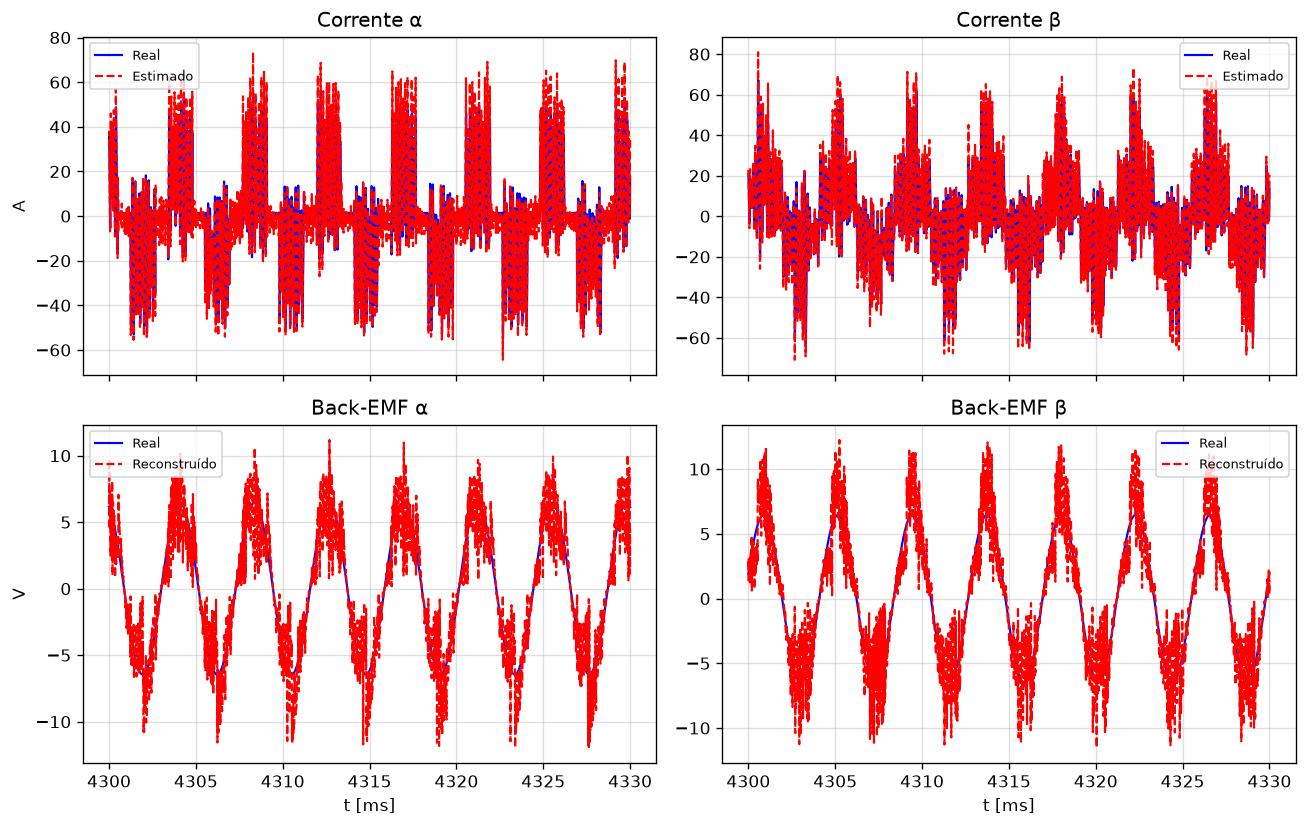
\includegraphics[width=0.9\linewidth]{Textuais/Imgs/Desenvolvimento/Eixo_alpha_beta.png}
    \label{fig:eixos_estaticos}

    Fonte: Autor (2026).
\end{figure}

Em síntese, os resultados de simulação evidenciam a eficácia da topologia
híbrida adotada para a estimação de estados. A integração do PLL com a
reconstrução analítica da força contraeletromotriz mostrou-se eficaz para
mitigar o \textit{chattering} intrínseco ao SMO e para evitar os atrasos
temporais de filtros passa-baixas convencionais, reduzindo o erro de fase a
poucos graus dentro do envelope de velocidade simulado. Encerrada a etapa
computacional, a modelagem foi traduzida para C e submetida aos registros de
bancada, tratados na \autoref{sec:ensaios_bancada}.

\newpage

\subsection{Identificação dos Coeficientes Aerodinâmicos Globais}
\label{sec:coef_aero}

O coeficiente de carga agrupa densidade do ar, diâmetro e coeficiente de
torque da hélice numa constante, $T = k_Q\,\omega_m^2$. Ele é identificado nos
patamares de rotação constante do perfil simulado, pelo mesmo procedimento do
ensaio de bancada (\autoref{fig:fluxo_ensaio_helice}), com as duas hélices
da \autoref{tab:parametros_simulacao}.

O torque de cada patamar é calculado com as correntes medidas projetadas no
ângulo estimado (\autoref{eq:torque_corrente_medida}), de modo que o
observador entra só com o ângulo e a velocidade. O coeficiente estimado
fica próximo do nominal nas duas hélices, com erro médio de
\SI{0,45}{\percent} na 15x6E e de \SI{0,32}{\percent} na 17x10E
(\autoref{tab:resultado_identificacao_cq} e \autoref{fig:patamar_coeff_CQ}).
O maior desvio, de cerca de \SI{3}{\percent} nas duas, aparece no último
patamar, logo após a desaceleração de \SIrange{5000}{3000}{RPM}; nos patamares
de subida o erro fica abaixo de \SI{1}{\percent},
mesmo com o torque médio dos patamares mais baixos de vinte a trinta vezes
menor que a amplitude da ondulação do acionamento em seis passos
(\autoref{fig:desempenho_mecanico}).

\begin{table}[H]
    \centering
    \caption{Identificação do coeficiente $k_Q$ por patamar}
    \label{tab:resultado_identificacao_cq}
    \small
    \setlength{\tabcolsep}{3pt}
    \begin{tabular}{ccccc}
        \toprule
        & \multicolumn{2}{c}{\textbf{APC 15x6E}} & \multicolumn{2}{c}{\textbf{APC 17x10E}} \\
        \cmidrule(lr){2-3} \cmidrule(lr){4-5}
        \textbf{RPM} &
        \textbf{$\bar{T}$ real / est. [\si{\newton\meter}]} &
        \textbf{$k_{Q}$ real / est. [$10^{-6}$]} &
        \textbf{$\bar{T}$ real / est. [\si{\newton\meter}]} &
        \textbf{$k_{Q}$ real / est. [$10^{-6}$]} \\
        \midrule
        1500 & \num{0,0452} / \num{0,0451} & \num{0,995} / \num{0,998} & \num{0,0850} / \num{0,0848} & \num{2,60} / \num{2,61} \\
        2000 & \num{0,0660} / \num{0,0659} & \num{0,995} / \num{0,997} & \num{0,1365} / \num{0,1365} & \num{2,60} / \num{2,61} \\
        2500 & \num{0,0924} / \num{0,0922} & \num{0,998} / \num{0,998} & \num{0,2022} / \num{0,2019} & \num{2,60} / \num{2,60} \\
        3000 & \num{0,1242} / \num{0,1243} & \num{0,998} / \num{1,00}  & \num{0,2823} / \num{0,2820} & \num{2,60} / \num{2,60} \\
        3500 & \num{0,1616} / \num{0,1612} & \num{0,999} / \num{0,999} & \num{0,3767} / \num{0,3756} & \num{2,60} / \num{2,60} \\
        4000 & \num{0,2042} / \num{0,2041} & \num{0,998} / \num{1,00}  & \num{0,4851} / \num{0,4841} & \num{2,60} / \num{2,60} \\
        4500 & \num{0,2527} / \num{0,2521} & \num{1,00} / \num{0,999}  & \num{0,6079} / \num{0,6064} & \num{2,60} / \num{2,60} \\
        5000 & \num{0,3062} / \num{0,3060} & \num{0,999} / \num{1,00}  & \num{0,7450} / \num{0,7380} & \num{2,60} / \num{2,58} \\
        3000\textsuperscript{a} & \num{0,1243} / \num{0,1241} & \num{0,998} / \num{0,968} & \num{0,2823} / \num{0,2824} & \num{2,60} / \num{2,52} \\
        \midrule
        \textbf{Est./nom.} & \multicolumn{2}{c}{\num{0,996} / \num{1,00} (\SI{0,45}{\percent})} &
            \multicolumn{2}{c}{\num{2,59} / \num{2,60} (\SI{0,32}{\percent})} \\
        \bottomrule
    \end{tabular}

    \vspace{2pt}
    {\footnotesize \textsuperscript{a} Patamar após a desaceleração de \SIrange{5000}{3000}{RPM}.}

    \vspace{0.2cm}
    {\small Fonte: Autor (2026)}
\end{table}

\begin{figure}[H]
    \centering
    \caption{Identificação do coeficiente $k_Q$ por patamar, por hélice}
    \label{fig:patamar_coeff_CQ}
    \begin{subfigure}[t]{\textwidth}
        \centering
        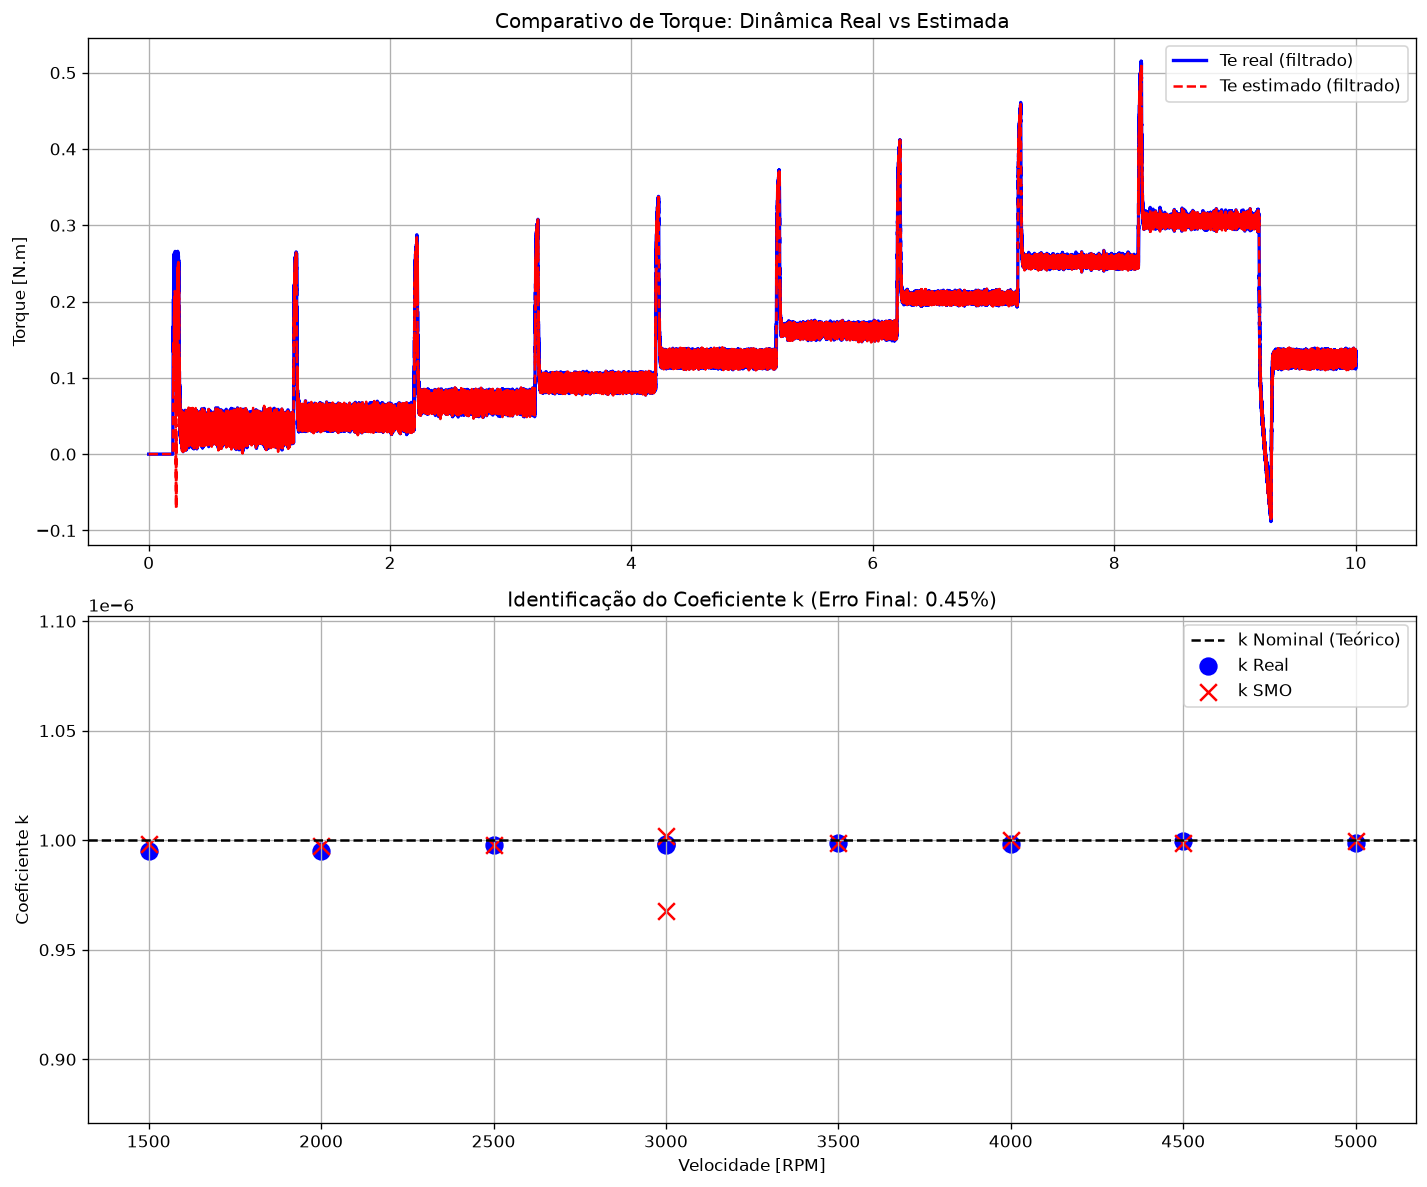
\includegraphics[width=0.8\linewidth]{Textuais/Imgs/Desenvolvimento/Algortimo_Coeficiente_helice_15x6E.png}
        \caption{APC 15x6E}
    \end{subfigure}

    \vspace{0.3cm}
    \begin{subfigure}[t]{\textwidth}
        \centering
        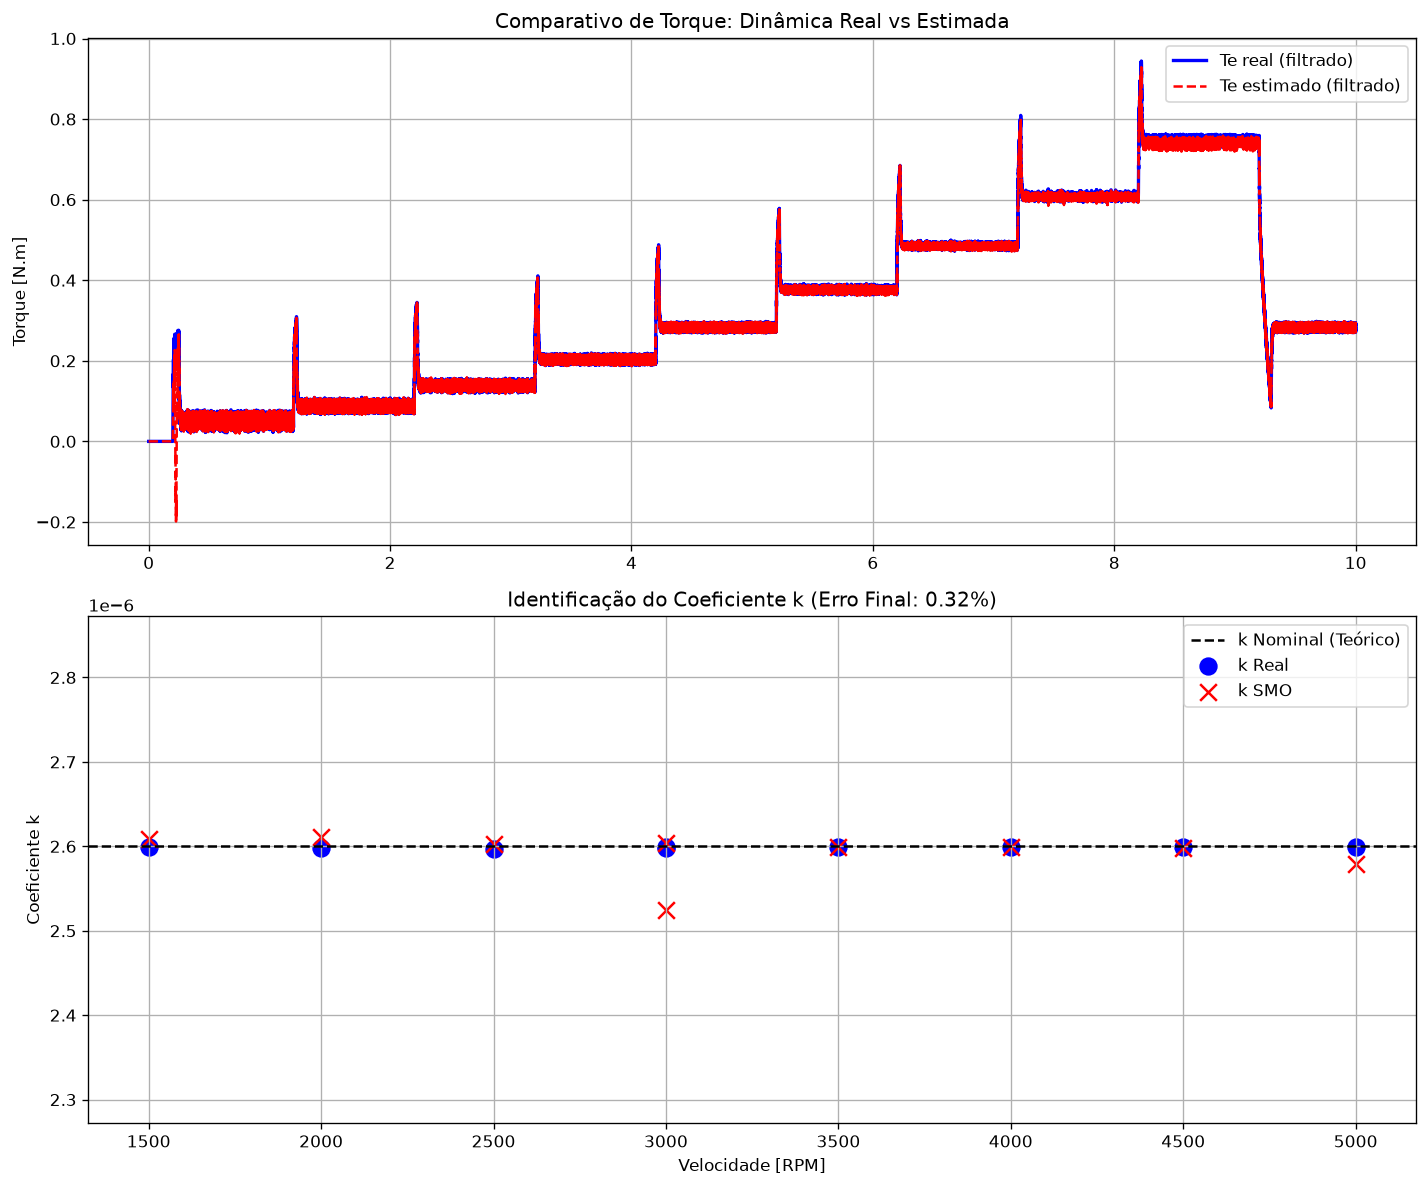
\includegraphics[width=0.8\linewidth]{Textuais/Imgs/Desenvolvimento/Algortimo_Coeficiente_helice_17x10E.png}
        \caption{APC 17x10E}
    \end{subfigure}

    Fonte: Autor (2026)
\end{figure}

\subsection{Coeficiente de Torque das Hélices em Bancada}
\label{sec:resultado_coef_aero_bancada}

As hélices APC 15x6E e 17x10E foram ensaiadas na condição estática do
procedimento da \autoref{sec:coef_aero_bancada}, com bateria de seis células.
O acelerador foi levado a três patamares, \SIlist{20;30;40}{\percent}, de
\SI{10}{\second} cada; em cada patamar, descartados os \SI{3}{\second}
iniciais de transitório, a rotação e o torque estimados pelo observador
embarcado foram promediados. O torque da hélice é o estimado menos as perdas a
vazio, $B\,\omega + \tau_c$ (\autoref{sec:resultado_coef_mec}), e $C_Q$ usa
$\rho = \SI{1,225}{\kilo\gram\per\cubic\meter}$. O teórico é a tabela do
fabricante na razão de avanço nula, com $C_Q$ obtido de $C_P$ pela
\autoref{eq:cq_from_cp}. A \autoref{tab:helice_15x6E} e a
\autoref{tab:helice_17x10E} dão os valores e o erro em relação ao teórico; a
\autoref{fig:helice_torque} e a \autoref{fig:helice_cq} mostram as mesmas
grandezas contra a rotação.

\begin{table}[H]
    \centering
    \caption{Torque e coeficiente $C_Q$ da hélice APC 15x6E na condição estática: teórico e bancada}
    \label{tab:helice_15x6E}
    \small
    \setlength{\tabcolsep}{4pt}
    \begin{tabular}{ccccccc}
        \toprule
        & & \multicolumn{2}{c}{\textbf{$Q$ [\si{\newton\meter}]}} & \multicolumn{2}{c}{\textbf{$C_Q$}} & \\
        \cmidrule(lr){3-4}\cmidrule(lr){5-6}
        \textbf{Acelerador} & \textbf{Rotação [RPM]} & \textbf{Teórico} & \textbf{Bancada} & \textbf{Teórico} & \textbf{Bancada} & \textbf{Erro} \\
        \midrule
        \SI{20}{\percent} & \num{1770} & \num{0,0358} & \num{0,0504} $\pm$ \num{0,0034} & \num{0,00418} & \num{0,00589} $\pm$ \num{0,00041} & \SI{+40,7}{\percent} \\
        \SI{30}{\percent} & \num{3050} & \num{0,0953} & \num{0,1191} $\pm$ \num{0,0052} & \num{0,00375} & \num{0,00469} $\pm$ \num{0,00022} & \SI{+25,0}{\percent} \\
        \SI{40}{\percent} & \num{3937} & \num{0,1545} & \num{0,1862} $\pm$ \num{0,0071} & \num{0,00365} & \num{0,00440} $\pm$ \num{0,00019} & \SI{+20,6}{\percent} \\
        \bottomrule
    \end{tabular}

    \vspace{2pt}
    {\small Fonte: Autor (2026); teórico adaptado de \citeonline{apc_performance_data}}
\end{table}

\begin{table}[H]
    \centering
    \caption{Torque e coeficiente $C_Q$ da hélice APC 17x10E na condição estática: teórico e bancada}
    \label{tab:helice_17x10E}
    \small
    \setlength{\tabcolsep}{4pt}
    \begin{tabular}{ccccccc}
        \toprule
        & & \multicolumn{2}{c}{\textbf{$Q$ [\si{\newton\meter}]}} & \multicolumn{2}{c}{\textbf{$C_Q$}} & \\
        \cmidrule(lr){3-4}\cmidrule(lr){5-6}
        \textbf{Acelerador} & \textbf{Rotação [RPM]} & \textbf{Teórico} & \textbf{Bancada} & \textbf{Teórico} & \textbf{Bancada} & \textbf{Erro} \\
        \midrule
        \SI{20}{\percent} & \num{1335} & \num{0,0573} & \num{0,0688} $\pm$ \num{0,0037} & \num{0,00630} & \num{0,00756} $\pm$ \num{0,00043} & \SI{+20,0}{\percent} \\
        \SI{30}{\percent} & \num{2308} & \num{0,1512} & \num{0,1758} $\pm$ \num{0,0066} & \num{0,00556} & \num{0,00646} $\pm$ \num{0,00027} & \SI{+16,3}{\percent} \\
        \SI{40}{\percent} & \num{3010} & \num{0,2431} & \num{0,2888} $\pm$ \num{0,0099} & \num{0,00525} & \num{0,00624} $\pm$ \num{0,00025} & \SI{+18,8}{\percent} \\
        \bottomrule
    \end{tabular}

    \vspace{2pt}
    {\small Fonte: Autor (2026); teórico adaptado de \citeonline{apc_performance_data}}
\end{table}

% Pontos medidos: Textuais/Imgs/Resultados/helice/medido_<hélice>.dat (torque do
% observador já corrigido para o divisor de 9,1 kOhm). Perdas: B = 32,4e-6 N.m.s/rad,
% tau_c = 15,5e-3 N.m. D^5: 15" = 8,028e-3 m^5; 17" = 1,5011e-2 m^5.
\pgfplotsset{
    helice/.style={width=\linewidth, height=5.5cm, grid=both,
        grid style={dotted,gray!40}, xmin=1000, xtick distance=1000, legend pos=north west,
        legend style={font=\scriptsize}, tick label style={font=\scriptsize},
        label style={font=\small}, xlabel={Rotação [RPM]},
        scaled x ticks=false, xticklabel style={/pgf/number format/1000 sep={}}},
    tabhelice/.style={table/comment chars={\#}},
    apcfaixa/.style={restrict x to domain=1000:4000},
    barras/.style={error bars/.cd, x dir=both, x explicit, y dir=both, y explicit,
        error bar style={line width=0.8pt}, error mark options={rotate=90, mark size=3pt, line width=0.8pt}},
}

\begin{figure}[H]
    \centering
    \caption{Torque aerodinâmico das hélices na condição estática: teórico e bancada}
    \label{fig:helice_torque}
    \begin{subfigure}[t]{0.49\textwidth}
        \centering
        \begin{tikzpicture}
        \begin{axis}[helice, xmax=4000, ylabel={$Q$ [\si{\newton\meter}]}, ymin=0]
            \addplot[thick, blue!65!black, apcfaixa] table[x=rpm, y=torque_Nm] {Textuais/Imgs/Resultados/helice/apc_15x6E_estatico.dat};
            \addlegendentry{APC (teórico)}
            \addplot[only marks, mark=*, blue!65!black, barras] table[tabhelice, x=rpm,
                y expr={\thisrow{Te_Nm} - (32.4e-6*\thisrow{rpm}*0.1047198 + 15.5e-3)},
                x error=rpm_err, y error expr={sqrt(\thisrow{Te_err}^2 + (0.03*\thisrow{Te_Nm})^2 + (4.4e-6*\thisrow{rpm}*0.1047198)^2 + (2.4e-3)^2)}]
                {Textuais/Imgs/Resultados/helice/medido_15x6E.dat};
            \addlegendentry{bancada}
        \end{axis}
        \end{tikzpicture}
        \caption{APC 15x6E}
    \end{subfigure}
    \hfill
    \begin{subfigure}[t]{0.49\textwidth}
        \centering
        \begin{tikzpicture}
        \begin{axis}[helice, xmax=4000, ylabel={$Q$ [\si{\newton\meter}]}, ymin=0]
            \addplot[thick, red!65!black, apcfaixa] table[x=rpm, y=torque_Nm] {Textuais/Imgs/Resultados/helice/apc_17x10E_estatico.dat};
            \addlegendentry{APC (teórico)}
            \addplot[only marks, mark=square*, red!65!black, barras] table[tabhelice, x=rpm,
                y expr={\thisrow{Te_Nm} - (32.4e-6*\thisrow{rpm}*0.1047198 + 15.5e-3)},
                x error=rpm_err, y error expr={sqrt(\thisrow{Te_err}^2 + (0.03*\thisrow{Te_Nm})^2 + (4.4e-6*\thisrow{rpm}*0.1047198)^2 + (2.4e-3)^2)}]
                {Textuais/Imgs/Resultados/helice/medido_17x10E.dat};
            \addlegendentry{bancada}
        \end{axis}
        \end{tikzpicture}
        \caption{APC 17x10E}
    \end{subfigure}

    Fonte: Autor (2026)
\end{figure}

\begin{figure}[H]
    \centering
    \caption{Coeficiente de torque $C_Q$ das hélices na condição estática: teórico e bancada}
    \label{fig:helice_cq}
    \begin{subfigure}[t]{0.49\textwidth}
        \centering
        \begin{tikzpicture}
        \begin{axis}[helice, xmax=4000, ylabel={$C_Q$}, ymin=0.003, ymax=0.0068, legend pos=north east,
                     yticklabel style={/pgf/number format/fixed, /pgf/number format/precision=4}]
            \addplot[thick, blue!65!black, apcfaixa] table[x=rpm, y=CQ] {Textuais/Imgs/Resultados/helice/apc_15x6E_estatico.dat};
            \addlegendentry{APC (teórico)}
            \addplot[only marks, mark=*, blue!65!black, barras] table[tabhelice, x=rpm,
                y expr={(\thisrow{Te_Nm} - (32.4e-6*\thisrow{rpm}*0.1047198 + 15.5e-3)) / (\thisrow{rho}*(\thisrow{rpm}/60)^2*8.0283e-3)},
                x error=rpm_err,
                y error expr={sqrt(\thisrow{Te_err}^2 + (0.03*\thisrow{Te_Nm})^2 + (4.4e-6*\thisrow{rpm}*0.1047198)^2 + (2.4e-3)^2
                        + (0.02*(\thisrow{Te_Nm} - (32.4e-6*\thisrow{rpm}*0.1047198 + 15.5e-3)))^2) / (\thisrow{rho}*(\thisrow{rpm}/60)^2*8.0283e-3)}]
                {Textuais/Imgs/Resultados/helice/medido_15x6E.dat};
            \addlegendentry{bancada}
        \end{axis}
        \end{tikzpicture}
        \caption{APC 15x6E}
    \end{subfigure}
    \hfill
    \begin{subfigure}[t]{0.49\textwidth}
        \centering
        \begin{tikzpicture}
        \begin{axis}[helice, xmax=4000, ylabel={$C_Q$}, ymin=0.004, ymax=0.0085, legend pos=north east,
                     yticklabel style={/pgf/number format/fixed, /pgf/number format/precision=4}]
            \addplot[thick, red!65!black, apcfaixa] table[x=rpm, y=CQ] {Textuais/Imgs/Resultados/helice/apc_17x10E_estatico.dat};
            \addlegendentry{APC (teórico)}
            \addplot[only marks, mark=square*, red!65!black, barras] table[tabhelice, x=rpm,
                y expr={(\thisrow{Te_Nm} - (32.4e-6*\thisrow{rpm}*0.1047198 + 15.5e-3)) / (\thisrow{rho}*(\thisrow{rpm}/60)^2*1.50111e-2)},
                x error=rpm_err,
                y error expr={sqrt(\thisrow{Te_err}^2 + (0.03*\thisrow{Te_Nm})^2 + (4.4e-6*\thisrow{rpm}*0.1047198)^2 + (2.4e-3)^2
                        + (0.02*(\thisrow{Te_Nm} - (32.4e-6*\thisrow{rpm}*0.1047198 + 15.5e-3)))^2) / (\thisrow{rho}*(\thisrow{rpm}/60)^2*1.50111e-2)}]
                {Textuais/Imgs/Resultados/helice/medido_17x10E.dat};
            \addlegendentry{bancada}
        \end{axis}
        \end{tikzpicture}
        \caption{APC 17x10E}
    \end{subfigure}

    Fonte: Autor (2026)
\end{figure}

O torque e o $C_Q$ de bancada seguem a forma das curvas teóricas: o torque
cresce com a rotação e o $C_Q$ diminui levemente, nas duas hélices. Os valores,
porém, ficam acima do teórico, de \SIrange{16}{20}{\percent} na 17x10E e de
\SIrange{21}{41}{\percent} na 15x6E. Algumas considerações sobre essa
diferença:

\begin{itemize}
    \item o teórico é resultado de simulação do fabricante, não de ensaio, e
    tende a ser menos preciso em rotações baixas, onde o escoamento nas pás
    tem número de Reynolds menor;
    \item o erro maior está na rotação mais baixa da 15x6E, onde o torque da
    hélice é pequeno e as perdas a vazio descontadas pesam mais; um erro de
    poucos \si{\milli\newton\meter} nessas perdas muda muito o resultado;
    \item o torque vem das correntes estimadas pelo observador, que na
    simulação ficaram \SIrange{4}{12}{\percent} acima do real com a 17x10E
    (\autoref{sec:autotuning});
    \item os ensaios rodaram com o coeficiente do divisor de corrente de
    \SI{10}{\kilo\ohm}; os valores foram corrigidos para o divisor montado, de
    \SI{9,1}{\kilo\ohm} (fator \num{1,032});
    \item a densidade do ar não foi medida no dia, e a bancada não tem medida
    de torque independente no mesmo eixo, que separaria o erro da estimativa da
    diferença real da hélice.
\end{itemize}

As barras de erro somam o desvio-padrão no patamar, a incerteza de $B$ e
$\tau_c$, \SI{3}{\percent} no ganho dos sensores de corrente e, no $C_Q$,
\SI{2}{\percent} na densidade do ar. A \autoref{fig:helice_gui} mostra os dois
registros como aparecem na interface, a partir do degrau de \SI{20}{\percent},
o primeiro que põe o motor em rotação. As tensões e correntes são amostras
isoladas a \SI{10}{\hertz}, cada uma num instante qualquer do chaveamento, e
não a forma de onda.

\begin{figure}[H]
    \centering
    \caption{Registros dos ensaios das hélices exibidos na interface de usuário}
    \label{fig:helice_gui}
    \begin{subfigure}[t]{\textwidth}
        \centering
        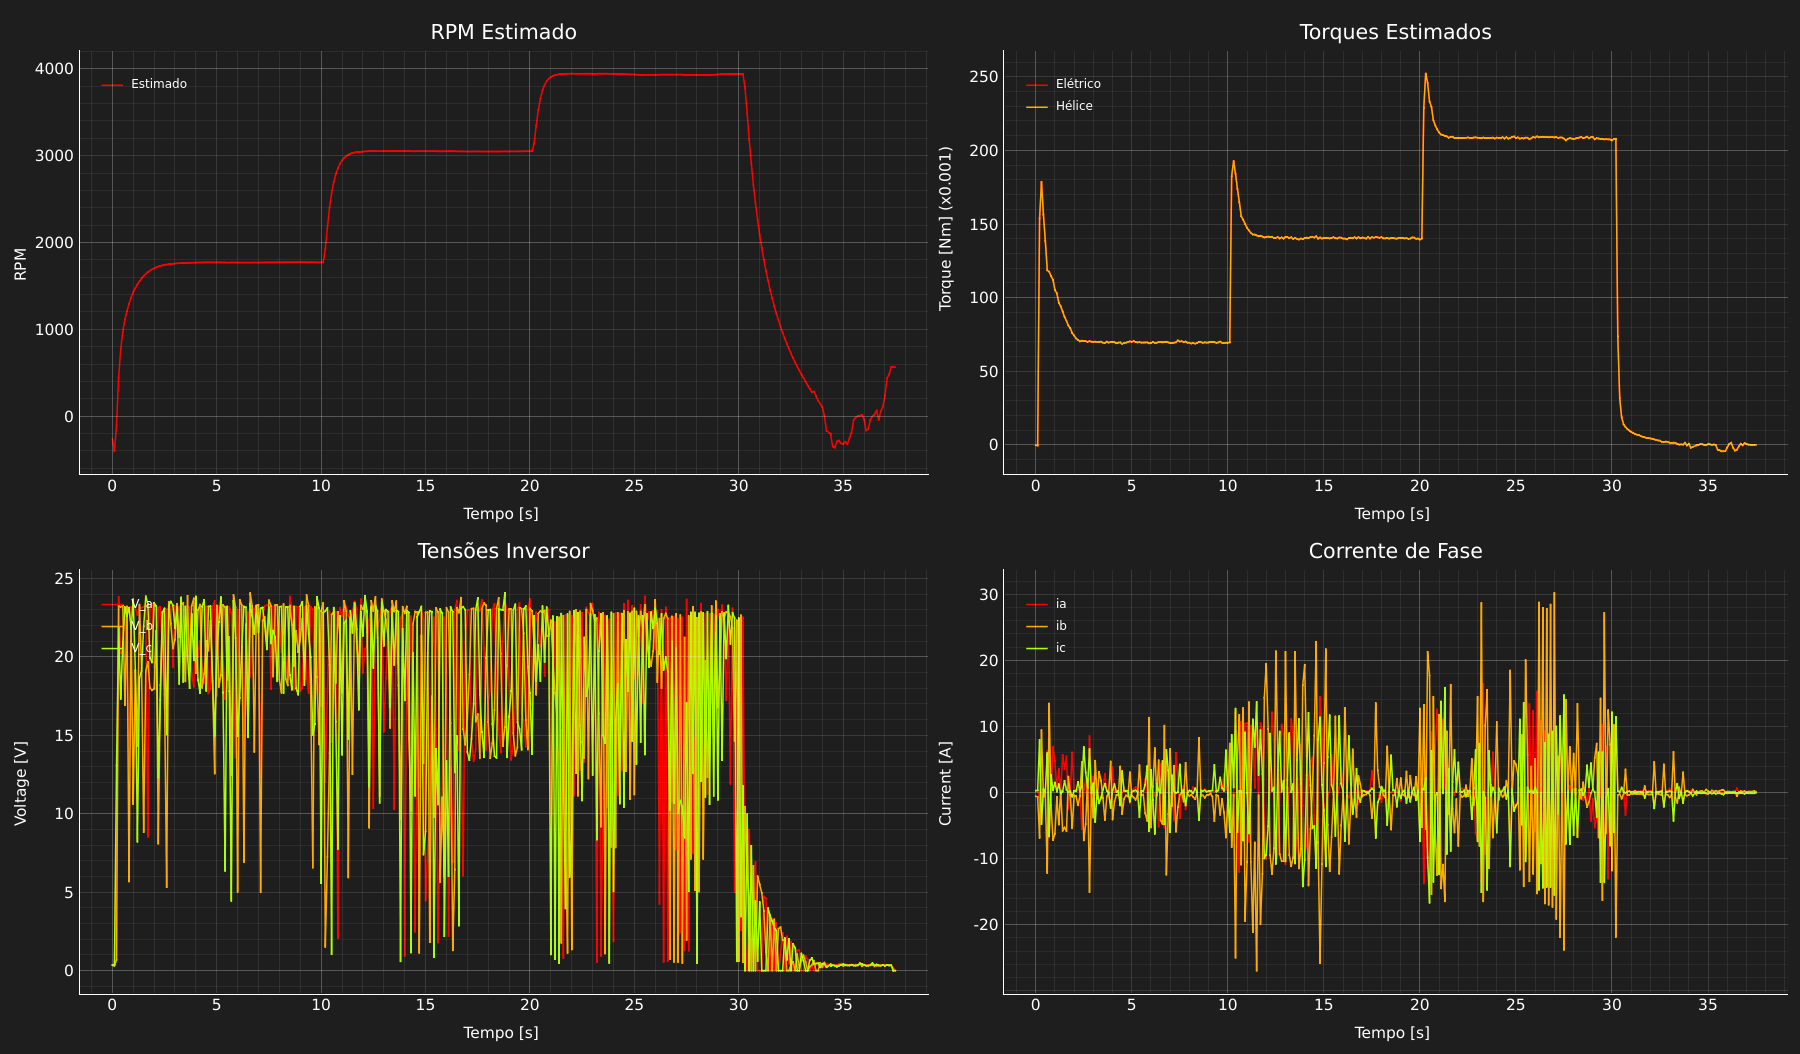
\includegraphics[width=0.95\linewidth]{Textuais/Imgs/Resultados/helice/gui_ensaio_15x6E.png}
        \caption{APC 15x6E}
    \end{subfigure}

    \vspace{0.3cm}
    \begin{subfigure}[t]{\textwidth}
        \centering
        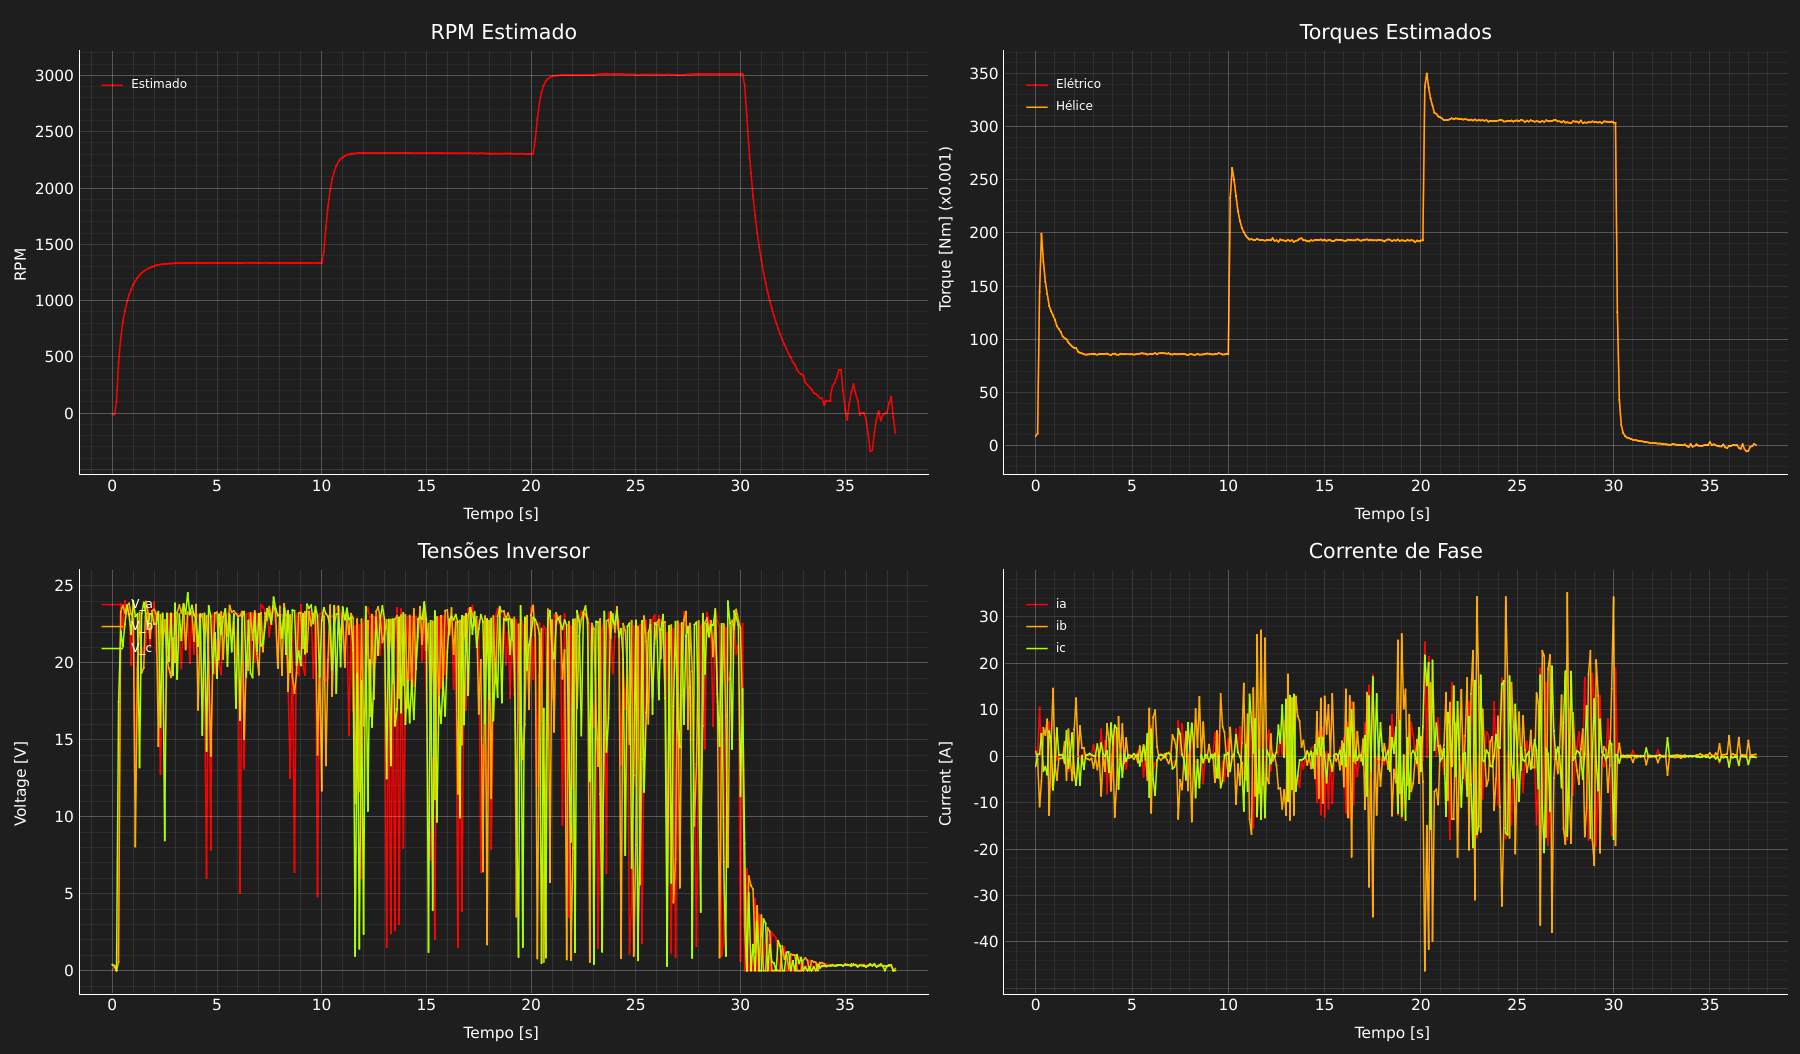
\includegraphics[width=0.95\linewidth]{Textuais/Imgs/Resultados/helice/gui_ensaio_17x10E.png}
        \caption{APC 17x10E}
    \end{subfigure}

    Fonte: Autor (2026)
\end{figure}
